\documentclass[12pt,a4paper]{article}

\usepackage[utf8]{inputenc}
\usepackage[T1]{fontenc}
\usepackage[brazilian]{babel}
\usepackage{lmodern}

\usepackage{amsmath,amssymb}
\usepackage{graphicx}
\usepackage{booktabs}
\usepackage{float}
\usepackage{geometry}
\usepackage{hyperref}

\geometry{margin=2.5cm}

\title{Relat\'orio -- Atividade 4\\Random Neurons vs. Random Forest}
\author{Caique Frederico Pereira de Moura\\ Aprendizado Computacional e Reconhecimento de Padr\~oes}
\date{\today}

\begin{document}
\maketitle

\section{Objetivo}
O objetivo desta atividade foi implementar o m\'etodo \emph{Random Neurons}, uma vers\~ao simplificada de \emph{Random Forest}, e avali\'a-lo em diferentes configura\c{c}\~oes de par\^ametros $L$ e $M$ nos conjuntos \emph{Iris} e \emph{Wine}. Em seguida, comparou-se o desempenho (percentual de acerto) com um \emph{Random Forest} configurado com $L$ \'arvores.

\section{M\'etodo: Random Neurons}
Considere um conjunto de treinamento $D = \{(\mathbf{x}_i,y_i) \in \mathbb{R}^n \times \{1,2,\dots,c\} : i=1,\dots,m\}$. O \emph{Random Neurons} foi implementado seguindo o roteiro proposto:

\begin{enumerate}
	\item \textbf{Bootstrap (bagging).} Para um dado $L \in \mathbb{N}$, foram geradas $L$ r\'eplicas $D_\ell$ de $D$ por amostragem com reposi\c{c}\~ao (bootstrap), com $\ell=1,\dots,L$.
	\item \textbf{Subespa\c{c}o aleat\'orio de atributos.} Para cada r\'eplica $D_\ell$, sorteou-se um inteiro $k \sim \mathcal{U}(\{1,\dots,n\})$ e selecionou-se, sem reposi\c{c}\~ao, um subconjunto de $k$ atributos. Os \i ndices sorteados foram armazenados para uso posterior.
	\item \textbf{Treinamento de classificadores base.} Para cada $\ell=1,\dots,L$, foi treinado um Perceptron de Bolso (\emph{Pocket Perceptron}) limitado a $M$ itera\c{c}\~oes, utilizando apenas o subconjunto de atributos sorteado para aquele modelo.
	\item \textbf{Multiclasse via OVR.} Como Iris e Wine s\~ao multiclasse, adotou-se \emph{one-vs-rest} (OVR): para cada classe $c$, ajusta-se um classificador bin\'ario que separa $c$ contra as demais.
	\item \textbf{Vota\c{c}\~ao por maioria.} Para classificar um padr\~ao $\mathbf{x}$, obteve-se a predi\c{c}\~ao de cada um dos $L$ modelos (com seus respectivos subconjuntos de atributos) e escolheu-se como sa\'ida a classe mais frequente.
\end{enumerate}

Em termos conceituais, o \emph{Random Neurons} combina \emph{bagging} com \emph{random subspace method}, trocando as \'arvores do Random Forest por classificadores lineares (Perceptron de Bolso), o que tende a aumentar o vi\'es do modelo quando a fronteira de decis\~ao \'e n\~ao linear.

\section{Protocolo experimental}
Os experimentos foram realizados conforme a implementa\c{c}\~ao em Python:\vspace{2mm}

\begin{itemize}
	\item \textbf{Bases de dados:} \emph{Iris} e \emph{Wine} (\texttt{sklearn.datasets}).
	\item \textbf{Divis\~ao treino-teste:} 70\%/30\% com \texttt{random\_state=42}.
	\item \textbf{Pr\'e-processamento:} padroniza\c{c}\~ao (\texttt{StandardScaler}) ajustada no treino e aplicada no teste.
	\item \textbf{Par\^ametros avaliados (Random Neurons):} $L \in \{5,10,20\}$ e $M \in \{50,100,200\}$.
	\item \textbf{Baseline (Random Forest):} \texttt{n\_estimators = L}, \texttt{max\_depth=None}, \texttt{min\_samples\_split=2}, \texttt{random\_state=42}.
	\item \textbf{M\'etrica:} acur\'acia no conjunto de teste.
\end{itemize}


\paragraph{Pré-processamento e reprodutibilidade.}
Os dados foram normalizados utilizando \emph{StandardScaler}, etapa essencial para o bom desempenho de modelos lineares como o Perceptron. Além disso, foi fixada uma semente pseudoaleatória (\texttt{random\_state = 42}) para garantir reprodutibilidade dos experimentos.

\paragraph{Configuração do Random Forest.}
O Random Forest foi configurado com $n\_estimators = L$, $max\_depth = None$ e $min\_samples\_split = 2$. A escolha de $max\_depth=None$ permite o crescimento completo das árvores, maximizando sua capacidade de modelagem e servindo como um comparativo forte em relação ao método proposto.

\section{Resultados}
As Tabelas~\ref{tab:iris} e~\ref{tab:wine} apresentam os percentuais de acerto observados para o \emph{Random Neurons}. Para o \emph{Random Forest}, a acur\'acia obtida para cada $L$ (com $L$ \'arvores) est\'a indicada na \'ultima coluna.

\begin{table}[H]
\centering
\caption{Iris: acur\'acia (\%) para diferentes $L$ e $M$.}
\label{tab:iris}
\begin{tabular}{@{}lrrrr@{}}
\toprule
\textbf{Configura\c{c}\~ao} & \textbf{$M=50$} & \textbf{$M=100$} & \textbf{$M=200$} & \textbf{RF ($L$ \'arvores)} \\
\midrule
$L=5$  & 82.22 & 91.11 & 77.78 & 100.00 \\
$L=10$ & 86.67 & 88.89 & 75.56 & 100.00 \\
$L=20$ & 88.89 & 84.44 & 75.56 & 100.00 \\
\bottomrule
\end{tabular}
\end{table}

\begin{table}[H]
\centering
\caption{Wine: acur\'acia (\%) para diferentes $L$ e $M$.}
\label{tab:wine}
\begin{tabular}{@{}lrrrr@{}}
\toprule
\textbf{Configura\c{c}\~ao} & \textbf{$M=50$} & \textbf{$M=100$} & \textbf{$M=200$} & \textbf{RF ($L$ \'arvores)} \\
\midrule
$L=5$  & 94.44 & 100.00 & 96.30 & 92.59 \\
$L=10$ & 96.30 & 100.00 & 98.15 & 92.59 \\
$L=20$ & 100.00 & 100.00 & 100.00 & 96.30 \\
\bottomrule
\end{tabular}
\end{table}

As Figuras 1 e 2 sintetizam os resultados, mostrando como a acur\'acia varia com $M$ e comparando com a linha de refer\^encia do \emph{Random Forest} para cada $L$.

\begin{figure}[H]
\centering
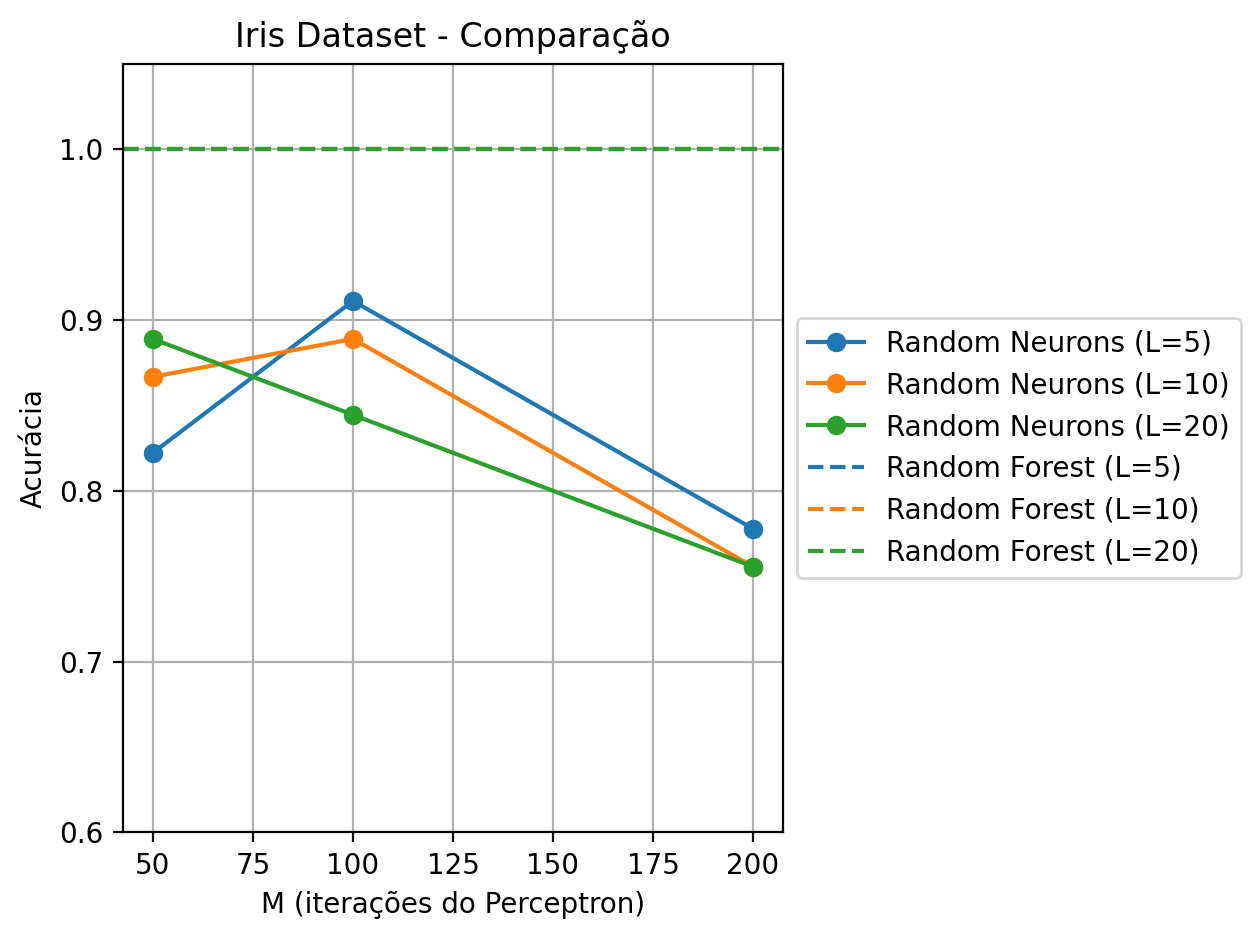
\includegraphics[width=0.85\textwidth]{images/iris.png}
\caption{Iris: compara\c{c}\~ao entre Random Neurons e Random Forest.}
\label{fig:iris}
\end{figure}

\begin{figure}[H]
\centering
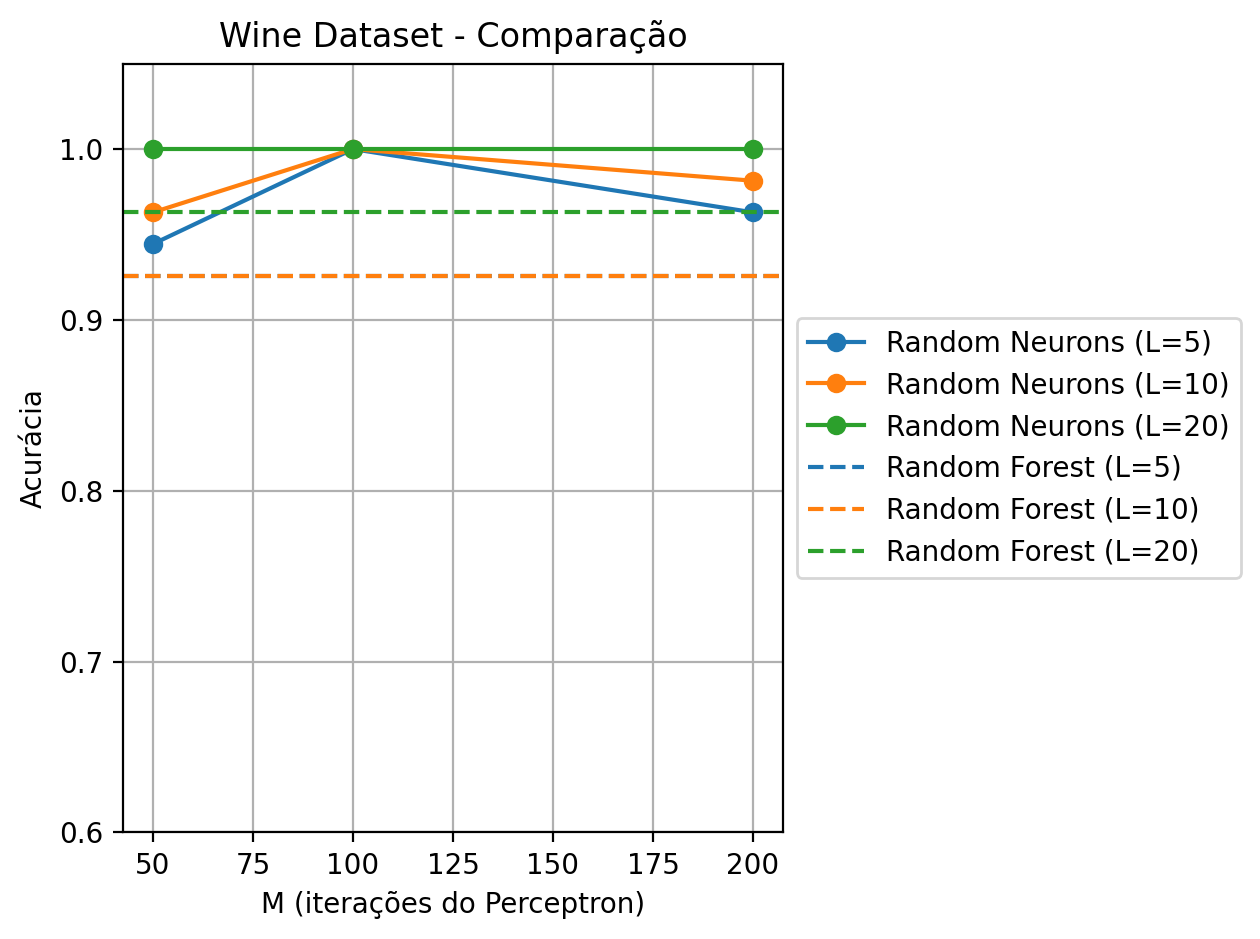
\includegraphics[width=0.85\textwidth]{images/wine.png}
\caption{Wine: compara\c{c}\~ao entre Random Neurons e Random Forest.}
\label{fig:wine}
\end{figure}

\section{Discuss\~ao}
No \emph{Iris}, o Random Forest obteve 100\% de acur\'acia para os valores de $L$ avaliados, enquanto o Random Neurons variou de aproximadamente 75.56\% a 91.11\%. Esse resultado \'e consistente com o fato de que o Random Neurons utiliza apenas classificadores lineares (Perceptron), o que imp\~oe maior vi\'es e pode n\~ao capturar fronteiras de decis\~ao n\~ao lineares. Al\'em disso, o sorteio aleat\'orio de atributos pode produzir subconjuntos pouco informativos, degradando o desempenho.

No \emph{Wine}, o comportamento foi distinto: o Random Neurons atingiu 100\% de acur\'acia em diversas configura\c{c}\~oes (por exemplo, $M=100$ para $L=5$, $L=10$ e $L=20$), superando o Random Forest em algumas delas. Isso sugere que, no Wine, existem subespa\c{c}os de atributos em que a separabilidade linear \'e alta e o ensemble (via bagging + subespa\c{c}os) consegue compensar a instabilidade de um classificador linear simples.

Quanto ao par\^ametro $M$, os resultados indicaram que aumentar o n\'umero m\'aximo de itera\c{c}\~oes do Perceptron nem sempre melhora a acur\'acia: em alguns casos, $M=200$ n\~ao trouxe ganhos e pode at\'e reduzir o desempenho, possivelmente por oscila\c{c}\~oes no ajuste e sensibilidade \`a amostra bootstrap e ao subespa\c{c}o sorteado.

\section{Conclus\~ao}
Os experimentos mostraram que o Random Forest \'e, em geral, mais robusto e confi\'avel (principalmente no Iris), enquanto o Random Neurons pode ser competitivo quando h\'a subespa\c{c}os linearmente separ\'aveis (como observado no Wine). Assim, o Random Neurons \'e uma alternativa interessante do ponto de vista did\'atico para discutir bagging, sele\c{c}\~ao aleat\'oria de atributos e vota\c{c}\~ao, mas n\~ao substitui m\'etodos mais expressivos em problemas com forte n\~ao linearidade.

\end{document}
